\section{Internet und IP-Adressen}

\begin{defi}{Internet}
    Das Internet, ist ein weltweiter Verbund von Rechnernetzwerken, den autonomen Systemen.
    Router werden als koppelnde Elemente zwischen den Teilnetzen genutzt.
\end{defi}

\begin{defi}{Netzwerk (ISO/OSI)}
    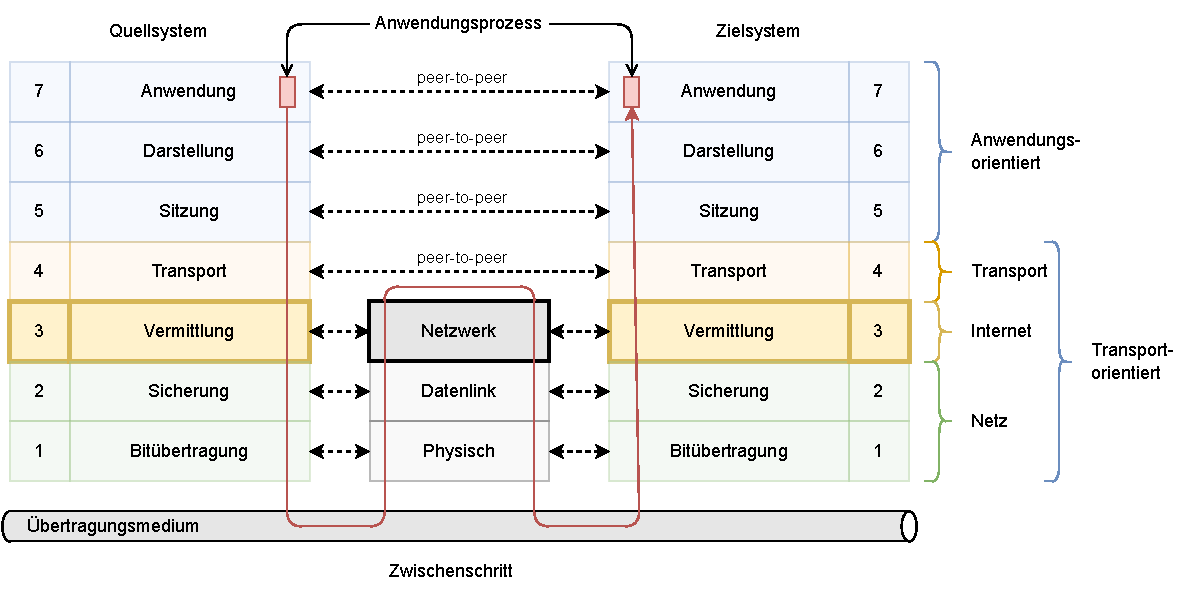
\includegraphics[width=\textwidth]{includes/figures/defi_iso_osi_network.pdf}
\end{defi}

\begin{defi}{TCP/IP}
    \emph{TCP/IP} ist eine protokollunabhängige Ausmodellierung des konzeptionellen \emph{ISO/OSI} Modells.

    \begin{center}
        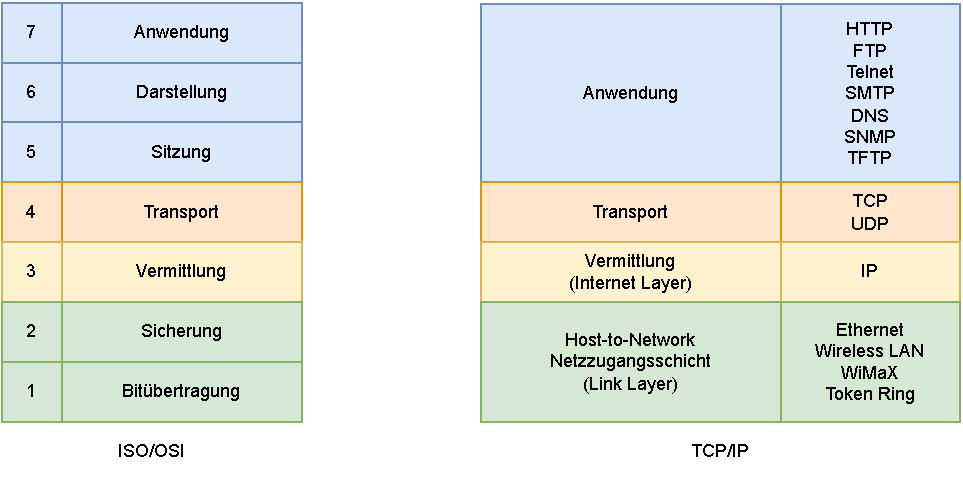
\includegraphics[width=0.75\textwidth]{includes/figures/defi_tcp_ip.pdf}
    \end{center}
\end{defi}

\begin{bonus}{Aufbau des Internets}
    Die Basis des Internets bilden \emph{Tier-1} Internet Service Provider (ISPs).
    Diese treten gleichberechtigt untereinander auf und sind durch vertraglich regulierte Verbindungen angebunden.

    Als Verbindung zwischen den ISPs dienen \emph{Network Access Points} (NAPs) oder \emph{Internet Exchange Points} (IXPs)

    \begin{center}
        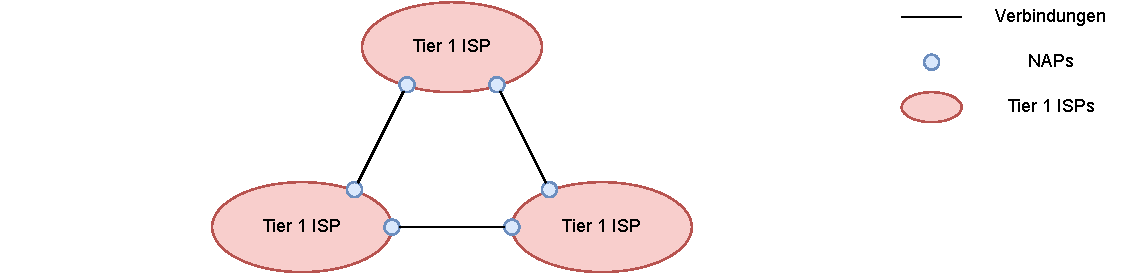
\includegraphics[width=0.75\textwidth]{includes/figures/bonus_aufbau_internet_1.pdf}
    \end{center}
\end{bonus}

\begin{bonus}{Aufbau des Internets}
    \emph{Tier 2} ISPs sind national bzw. regional und sind immer an einen oder mehrere \emph{Tier 1} ISPs angeschlossen.

    Sie treten dabei gegenüber \emph{Tier 1} ISPs als KundIn auf.

    \begin{center}
        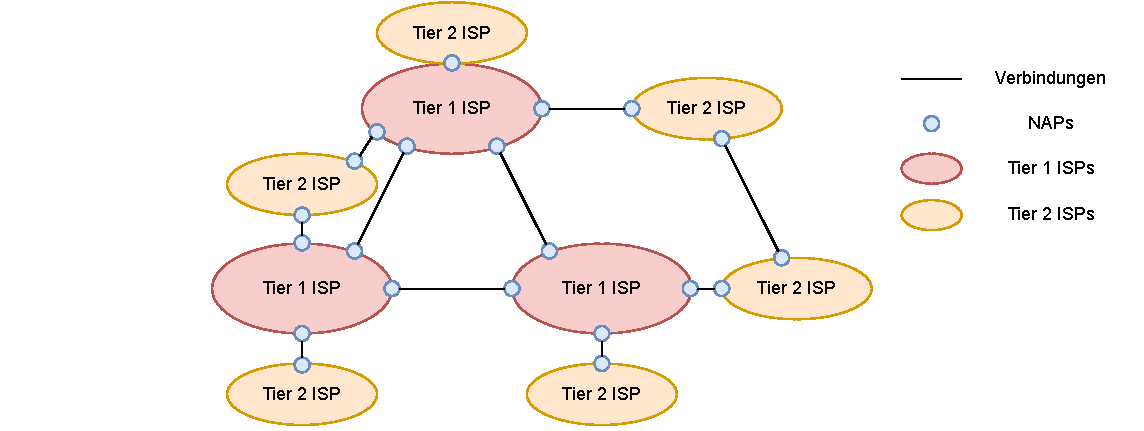
\includegraphics[width=0.75\textwidth]{includes/figures/bonus_aufbau_internet_2.pdf}
    \end{center}
\end{bonus}

\begin{bonus}{Aufbau des Internets}
    \emph{Tier 3} ISPs binden den Kunden beispielsweise über DSL direkt an das gesamte Netzwerk an.

    Sie treten dabei gegenüber \emph{Tier 2} ISPs selber als KundIn auf.

    \begin{center}
        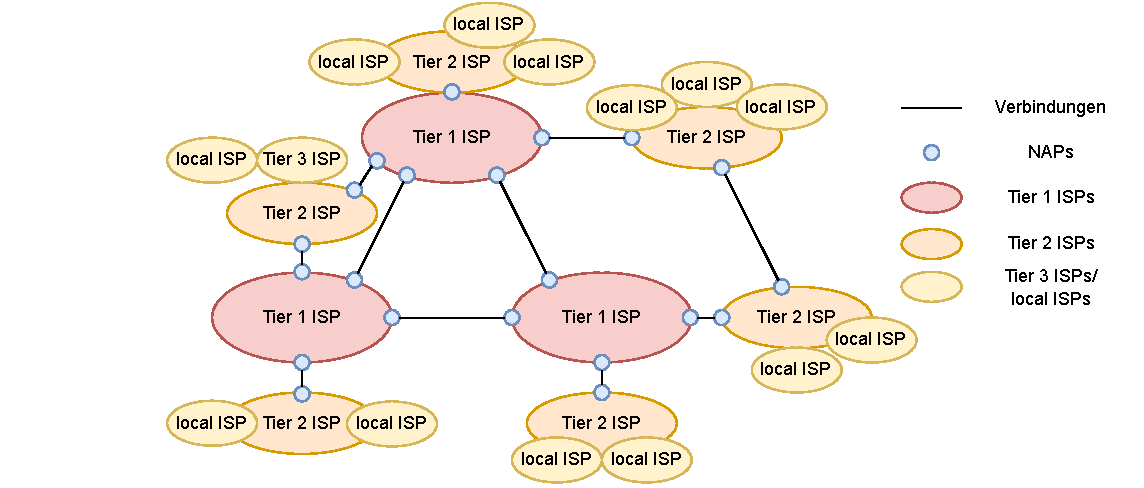
\includegraphics[width=0.75\textwidth]{includes/figures/bonus_aufbau_internet_3.pdf}
    \end{center}
\end{bonus}

\begin{bonus}{Aufbau des Internets}
    \begin{center}
        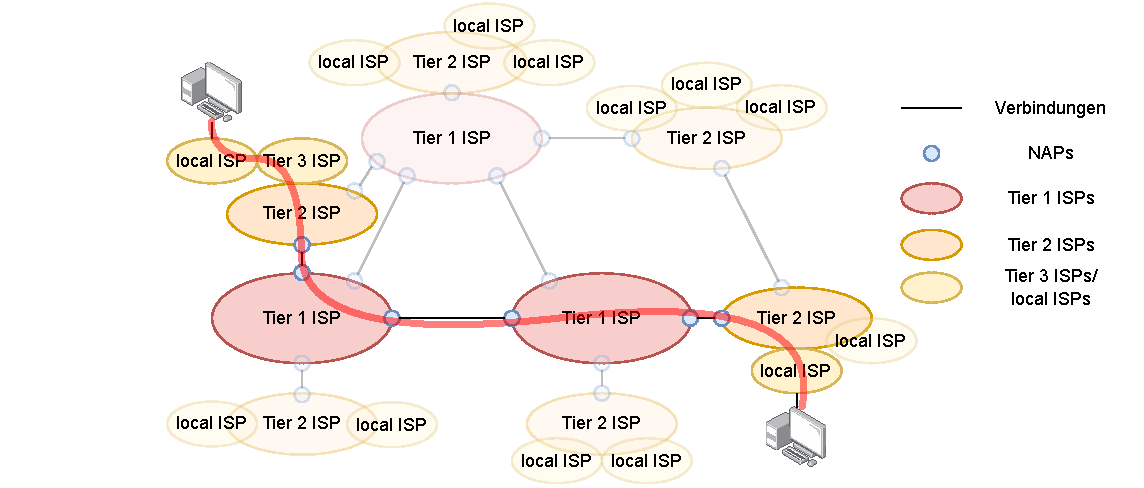
\includegraphics[width=0.75\textwidth]{includes/figures/bonus_aufbau_internet_4.pdf}
    \end{center}
\end{bonus}

\begin{bonus}{Nachrichtenzustellung}
    \begin{wrapfigure}{r}{0.25\textwidth}
        \begin{center}
            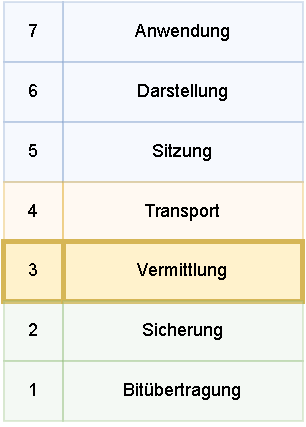
\includegraphics[width=0.2\textwidth]{includes/figures/bonus_iso_osi_vermittlung.pdf}
        \end{center}
    \end{wrapfigure}
    %
    Die Herausforderung in diesem großen Netz aus Netzen ist es Datenpakete von einem beliebigen Endgerät zu einem bestimmten Ziel zu versenden.

    Damit dies gelingt, wird in der Vermittlungsschicht einer der möglichen Wege zum Zielgerät gewählt.
    Die Wegwahl findet durch \emph{Routing Protokolle} statt.

    Die Entscheidung erfolgt durch \emph{Routing Tabellen}.
    In diesen lassen sich - je nach Protokoll - definierte Wege finden, unter denen man das autonome System des Zielgeräts findet bzw. welcher Weg befolgt werden soll, wenn das Zielgerät komplett unbekannt ist.

    In der Vermittlungsschicht wird größtenteils das IP-Protokoll genutzt, um die Pakete zu adressieren und Regeln zur Paketbehandlung aufzustellen.
\end{bonus}

\begin{defi}{Kapselung von Protokoll-Headern}
    Zur erfolgreichen Nachrichtenzustellung erweitern die verschiedenen Protokollinstanzen ein von einer Anwendung produziertes Datenpaket um verschiedene fest definierte Header.

    \begin{center}
        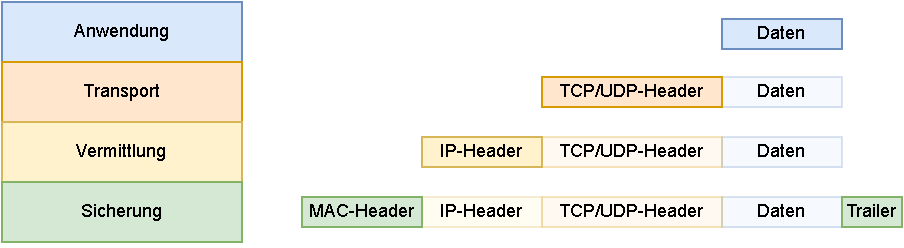
\includegraphics[width=0.75\textwidth]{includes/figures/defi_header_kapselung.pdf}
    \end{center}

    \begin{itemize}
        \item TCP bzw. UDP-Header dienen zur eindeutigen Prozessadressieren durch Ports.
        \item TCP sichert darüber hinaus die Datenübertragung
        \item IP-Header identifizieren ein eindeutiges Quell und Zielsystem
    \end{itemize}

    Demnach entsteht folgendes versandfertiges Datagramm:

    \begin{center}
        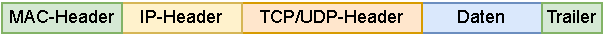
\includegraphics[width=0.75\textwidth]{includes/figures/defi_datagramm.pdf}
    \end{center}
\end{defi}

\begin{defi}{Das Internet-Protokoll (IP)}
    \emph{IP} bietet eine Ende-zu-Ende Kommunikation zwischen Endgeräten im Internet.
    Derzeit wird flächendeckend \emph{IPv4} bzw. \emph{IPv6} eingesetzt.

    IP ist paketvermittelnd, leitet also in sich geschlossene, unabhängige Dateneinheiten bzw. Datagramme ungesichert zwischen zwei Endpunkten weiter.
    Jedes Paket wird dabei in dem jeweiligen Router zwischengespeichert, überprüft und dementsprechend aussortiert oder weitergeleitet.
    Da die Pakete parallel von den Routern abgearbeitet werden, kann es passieren, dass:
    \begin{itemize}
        \item Datagramme verloren gehen
        \item Datagramme sich gegenseitig überholen
        \item Datagramme mehrfach ankommen
    \end{itemize}

    \emph{Sitzungen} werden durch einen exklusiven Kommunikationskanal über TCP simuliert.
\end{defi}

\begin{defi}{Wegwahl im Internet-Protokoll}
    Die IP-Implementierung eines Rechners oder Routers entscheidet eigenständig, wohin dieser ein Datagramm übertragen soll.

    Diese Entscheidung wird auf Basis von Routing bzw. Forwarding-Tabellen getroffen\footnote{Wie Routingtabellen aufgebaut werden, wird zu einem späteren Zeitpunkt erwähnt.}.
    Dazu werden die Informationen, normalerweise ausschließlich die Zieladresse des Pakets, aus dem IP-Header in der jeweiligen Tabelle abgefragt.

    Router sind dabei meist an mehreren Netzen angeschlossen.
    Sie müssen zusätzlich noch überprüfen, ob sich das Zielgerät in einem anderen Netz befindet als das Quellgerät bzw. wie dieses Netz erreicht werden kann.
\end{defi}

\begin{example}{Wegwahl im Internet Protokoll}
    In folgendem Beispiel möchte \emph{Rechner A} an Paket an \emph{Rechner F} senden.

    \begin{center}
        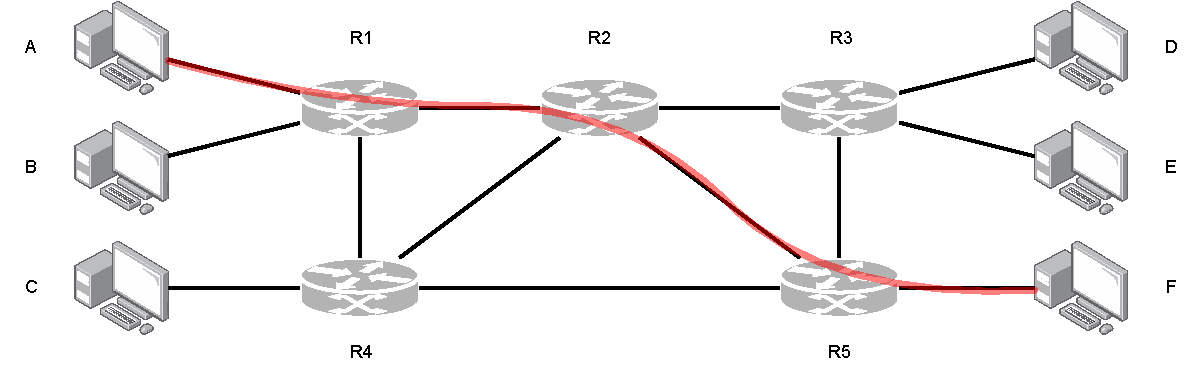
\includegraphics[width=0.75\textwidth]{includes/figures/example_ip_routing.pdf }
    \end{center}

    \begin{minipage}{0.25\textwidth}
        \begin{center}
            \emph{Rechner A}

            \begin{tabular}{|c|l|}
                \hline
                \textbf{Ziel} & \textbf{Next Hop} \\\hline
                *             & $\to$ R1          \\\hline
            \end{tabular}
        \end{center}
    \end{minipage}
    \begin{minipage}{0.25\textwidth}
        \begin{center}
            \emph{R1}

            \begin{tabular}{|c|l|}
                \hline
                \textbf{Ziel} & \textbf{Next Hop} \\\hline
                A             & A                 \\
                B             & B                 \\
                C             & R4                \\
                D             & R2                \\
                E             & R2                \\
                F             & $\to$ R2          \\\hline
            \end{tabular}
        \end{center}
    \end{minipage}
    \begin{minipage}{0.25\textwidth}
        \begin{center}
            \emph{R2}

            \begin{tabular}{|c|l|}
                \hline
                \textbf{Ziel} & \textbf{Next Hop} \\\hline
                A             & R1                \\
                B             & R1                \\
                C             & R4                \\
                D             & R3                \\
                E             & R3                \\
                F             & $\to$ R5          \\\hline
            \end{tabular}
        \end{center}
    \end{minipage}
    \begin{minipage}{0.25\textwidth}
        \begin{center}
            \emph{R5}

            \begin{tabular}{|c|l|}
                \hline
                \textbf{Ziel} & \textbf{Next Hop} \\\hline
                A             & R2                \\
                B             & R2                \\
                C             & R4                \\
                D             & R3                \\
                E             & R3                \\
                F             & $\to$ F           \\\hline
            \end{tabular}
        \end{center}
    \end{minipage}
\end{example}

\begin{defi}{IPv4-Adresse}
    Im Internet sind Endgeräte nicht über Namen erreichbar, sondern haben eine \emph{IP Adresse}.

    Diese sind 32 bit bzw. 4 Byte lang und sind unterteilt in einen Bereich um das Netz zu adressieren und einen Bereich um diesen Rechner in dem angegebenen Netz zu identifizieren.
    In Kombination ist die IP-Adresse (theoretisch) Weltweit eindeutig.

    Zur einfachen und übersichtlichen Darstellung werden IP-Adressen in vier Blöcke je ein Byte aufgeteilt, von denen jeder eine dezimale Zahl darstellt\footnote{Führende Nullen können bei der Visualisierung weggelassen werden.}:

    z.B. \texttt{134.130.0.0}\footnote{Class B Netz der RWTH Aachen University}
\end{defi}

\begin{defi}{IPv4-Adressklassen}
    Um die verfügbaren IP-Adressen fair und sinnvoll aufzuteilen, wurden \emph{Klassen} definiert.
    Mithilfe dieser Klassen können Anfragen von KundInnen, je nach benötigter Anzahl von IP-Adressen, schnell bearbeitet werden.

    \begin{enumerate}[label=Class \Alph*:, leftmargin=*]
        \item Für Netze mit bis zu 16 Mio Knoten

              (Knoten-ID: $0\text{-}127$, 50\% des IPv4-Adressraums)
    \end{enumerate}

    \begin{center}
        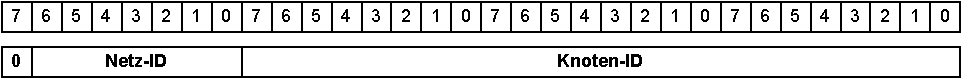
\includegraphics[width=0.75\textwidth]{includes/figures/bonus_class_a.pdf}
    \end{center}

    \begin{enumerate}[label=Class \Alph*:, leftmargin=*, start=2]
        \item Für Netze mit bis zu 65.536 Knoten

              (Knoten-ID: $128\text{-}191$, 25\% des IPv4-Adressraums)
    \end{enumerate}

    \begin{center}
        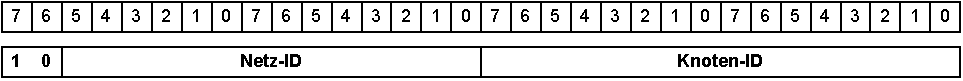
\includegraphics[width=0.75\textwidth]{includes/figures/bonus_class_b.pdf}
    \end{center}

    \begin{enumerate}[label=Class \Alph*:, leftmargin=*, start=3]
        \item Für Netze mit bis zu 256 Knoten

              (Knoten-ID: $192\text{-}223$, 12.5\% des IPv4-Adressraums)
    \end{enumerate}

    \begin{center}
        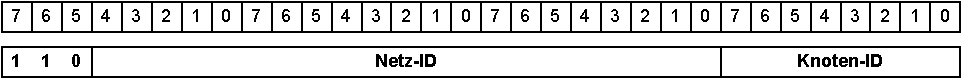
\includegraphics[width=0.75\textwidth]{includes/figures/bonus_class_c.pdf}
    \end{center}

    \begin{enumerate}[label=Class \Alph*:, leftmargin=*, start=4]
        \item Für Gruppenkommunikation

              (Knoten-ID: $224\text{-}239$, 6.25\% des IPv4-Adressraums)
    \end{enumerate}

    \begin{center}
        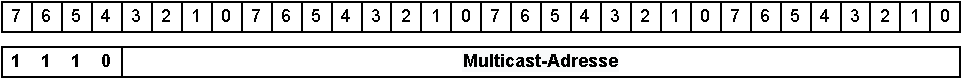
\includegraphics[width=0.75\textwidth]{includes/figures/bonus_class_d.pdf}
    \end{center}

    \begin{enumerate}[label=Class \Alph*:, leftmargin=*, start=5]
        \item Reserviert für zukünftige Anwendungen

              (Knoten-ID: $240\text{-}255$, 6.25\% des IPv4-Adressraums)
    \end{enumerate}

    \begin{center}
        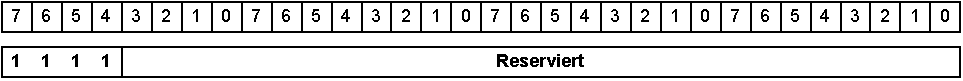
\includegraphics[width=0.75\textwidth]{includes/figures/bonus_class_e.pdf}
    \end{center}

    In allen Netzen ist die Koten-ID 0..0 ($0$) für das Netz selber reserviert.

    Des weiteren wird für Broadcast Nachrichten an alle teilnehmenden Geräte im Netz die Knoten-ID 1..1 ($\text{A: } 127 \text{ bzw. B: } 191 \text{ bzw. C: } 223$) genutzt
\end{defi}

\begin{bonus}{Probleme IPv4}
    Da nur ca. 4.3 Mrd. ($2^{32}$) Adressen zur Verfügung stehen, kann nicht jedes Gerät eine eigene weltweit eindeutige IP-Adresse erhalten.
    Anfänglich hatte niemand damit gerechnet, dass dieses neue Phänomen Internet derart stark wächst.

    Um dieses Problem zu lösen, bzw. die resultierenden Auswirkungen aufzuschieben, wurden private Netze eingeführt.
    Da ebenfalls festgestellt wurde, dass Adressklassen auf Grund hoher Verschwendung an überschüssigen IP Adressen nicht zielführend war\footnote{
        Wenn man mehr als 254 Endgeräte anschließen möchte, benötigt man bereits ein Klasse B Netz.
        Es bleiben bis zu 64.281 Adressen ungenutzt
    }, konnte man die Grenze zwischen Netz-ID und Knoten-ID nun beliebig wählen.
    Alternativ erhält man mehrere kleine Netze, die man durch Router Verbinden muss.

    Jedes IP Netz benötigt ab jetzt ebenfalls eine Subnetzmaske.
    Diese wird genutzt um eindeutig zwischen Netz und Knoten-ID zu unterscheiden.

    Die Subnetzmaske kann entweder in IPv4 oder in CIDR (Classless Inter-Domain Routing) Schreibweise angegeben werden.
    In CIDR wird die Anzahl der \texttt{1}en in der Subnetzmaske hinter der IPv4 Adresse angegeben. Die Stellen der Knoten-ID können weggelassen werden.

    Um eine gewisse Struktur in private Netze zu bringen, wurden gewisse Richtlinien geschaffen, um aus den historischen Klassen private Netze zu erstellen.
    Jedes übersetzte Netz hat 24 frei wählbare Stellen.
    Im Gegensatz dazu kann man in eigenen privaten Netzen alle Stellen der IP-Adresse frei wählen.
    Dabei entscheidet die Länge der Subnetzmaske ($\text{snm}$) über die Anzahl der verfügbaren IPv4-Adressen ($2^{32-\text{snm}}$).
    \begin{center}
        \begin{tabular}{|c|l|l|l|l|}
            \hline
            \textbf{Klasse} & \textbf{CIDR-Notation} & \textbf{Anzahl Netze} & \textbf{Anzahl Adressen} & \textbf{Netze}            \\\hline
            A               & \texttt{10/8}          & $2^0 = 1$             & $2^{24} = 16.777.216$    & \texttt{10/8}             \\\hline
            B               & \texttt{172.16/12}     & $2^4 = 16$            & $2^{20} = 1.048.576$     & \texttt{172.16/16} bis    \\
                            &                        &                       &                          & \texttt{172.31/16}        \\\hline
            C               & \texttt{192.168/16}    & $2^8 = 256$           & $2^{16} = 65.536$        & \texttt{192.168.0/24} bis \\
                            &                        &                       &                          & \texttt{192.168.255/24}   \\\hline
            /24             & \texttt{192.168.0/24}  &                       & $2^{32-24} = 2^8 = 256$  &                           \\\hline
        \end{tabular}
    \end{center}
\end{bonus}

\begin{example}{IPv4-Netz}
    Betrachten wir ein typisches IPv4-Netz mit Subnetzmaske:
    \texttt{192.168.0.0} mit \texttt{255.255.255.0}

    bzw. in CIDR:
    \texttt{192.168.0.0/24} bzw. \texttt{192.168.0/24}

    Wenn wir eine beliebige IP-Adresse aus diesem Netz erhalten, können wir mithilfe logischer Gatter zuerst das Netz eindeutig identifizieren, und dann den Host adressieren.

    z.B. \texttt{192.168.0.4/24}

    \begin{center}
        \begin{tabular}{|l|c|l|}
            \hline
            \textbf{IP-Adresse}                                                                                     & \texttt{1100 0000 . 1010 1000 . 0000 0000 . 0000 0100}          & \texttt{192.168.0.4}          \\\hline
            \textbf{Subnetzmaske}                                                                                   & \texttt{1111 1111 . 1111 1111 . 1111 1111 . 0000 0000}          & \texttt{255.255.255.0}        \\\hline
            \textbf{Netz-ID}\footnote{$\text{Netz-ID} = \text{IP-Adresse} \land \text{Subnetzmaske}$}               & \texttt{\textbf{1100 0000 . 1010 1000 . 0000 0000} . 0000 0000} & \texttt{\textbf{192.168.0}.0} \\\hline
            \textbf{Geräte-ID}\footnote{$\text{Geräte-ID} = \text{IP-Adresse} \land	\overline{\text{Subnetzmaske}}$} & \texttt{0000 0000 . 0000 0000 . 0000 0000 . \textbf{0000 0100}} & \texttt{0.0.0.\textbf{4}}     \\\hline
        \end{tabular}
    \end{center}
\end{example}

\begin{bonus}{Loopback-Adresse}
    Um Kommunikation mit Anwendungen auf dem selben Rechner zu führen, kann man die IPv4-Adresse \texttt{127.0.0.1} nutzen.
    Diese virtuelle Netzwerkkarte verfolgt nicht die tieferen Schichten des ISO-OSI Modells, sondern geht \enquote{zurück} über die Transportschicht an die angesprochene Anwendung.
\end{bonus}

\begin{defi}{IP-Subnetze}
    Wenn wir nun die bestehenden Netzwerkklassen mit unseren neuen bekannten Subnetzmasken zusammenfügen, können wir große Netze in kleine durch Router getrennte Bereiche aufteilen.

    Auf Grund des Präfix erkannt man an der IPv4-Adresse die Adressklasse.
    Anhand der Subnetzmaske erkennt man die Länge der Netz-ID.

    Stimmen die Längen der Netz-ID der Adressklasse und die Gesamtlänge der Netz-ID überein, haben wir keine Subnetze.
    Ist die Gesamtlänge der Netz-ID länger, können wir errechnen, wie viele Subnetze möglich sind.
\end{defi}

\begin{example}{IP-Subnetze}
    Nehmen wir das Klasse B Netz der RWTH Aachen University:
    \texttt{134.130.0.0}\footnote{
        Netz-Adresse startet in binär mit \texttt{10}.
        Daher wissen wir, dass es sich um ein Klasse B Netz handelt
    }

    In diesem Klasse B Netz befinden sich folgende Subnetze:\\
    \texttt{134.130.1.0/24}\\
    \texttt{134.130.2.0/24}\\
    \texttt{134.130.3.0/24}

    Durch die Subnetzmaske wissen wir, dass die Netz-ID die ein Byte länger ist, als die Netz-ID der Netzklasse.
    Dementsprechend können wir bis zu 256 Subnetze mit jeweils bis zu 254\footnote{
        Obacht: Die logische Aufteilung in Subnetze ist sinnvoll, jedoch gehen bei jedem Subnetz jeweils zwei IP-Adressen für Netz-Adresse und Broadcast verloren.
        Dementsprechend sollte man Subnetze ausschließlich für unabhängige Instanzen nutzen.
        z.B. Institute der RWTH, Dezernate der FH-Aachen etc.
    } Endgeräten erstellen.

    z.B. \texttt{134.130.1.4/24}

    \begin{center}
        \begin{tabular}{|l|c|l|}
            \hline
            \textbf{IP-Adresse}                                                                                                                     & \texttt{1000 0110 . 1000 0010 . 0000 0001 . 0000 0100}          & \texttt{134.130.1.4}          \\\hline
            \textbf{Subnetzmaske}                                                                                                                   & \texttt{1111 1111 . 1111 1111 . 1111 1111 . 0000 0000}          & \texttt{255.255.255.0}        \\\hline
            \textbf{IP-Klassenmaske}\footnote{Bekannt durch IP-Klassenpräfix}                                                                       & \texttt{1111 1111 . 1111 1111 . 0000 0000 . 0000 0000}          & \texttt{255.255.0.0}          \\\hline
            \textbf{Netz-ID}\footnote{$\text{Netz-ID} = \text{IP-Adresse} \land \text{Subnetzmaske} \land \text{IP-Klassenmaske}$}                  & \texttt{\textbf{1000 0110 . 1000 0010} . 0000 0000 . 0000 0000} & \texttt{\textbf{134.130}.0.0} \\\hline
            \textbf{Subnetz-ID}\footnote{$\text{Subnetz-ID} = \text{IP-Adresse} \land \text{Subnetzmaske} \land \overline{\text{IP-Klassenmaske}}$} & \texttt{0000 0000 . 0000 0000 . \textbf{0000 0001} . 0000 0000} & \texttt{0.0.\textbf{1}.0}     \\\hline
            \textbf{Geräte-ID}\footnote{$\text{Geräte-ID} = \text{IP-Adresse} \land	\overline{\text{Subnetzmaske}}$}                                 & \texttt{0000 0000 . 0000 0000 . 0000 0000 . \textbf{0000 0100}} & \texttt{0.0.0.\textbf{4}}     \\\hline
        \end{tabular}
    \end{center}
\end{example}

\begin{defi}{IP-Header}
    \begin{center}
        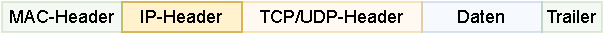
\includegraphics[width=0.75\textwidth]{includes/figures/defi_ip_header_kapselung.pdf}

        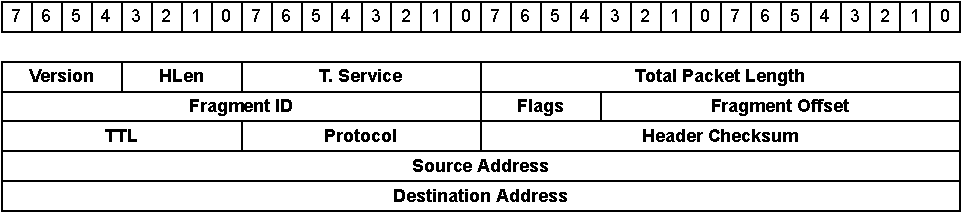
\includegraphics[width=0.75\textwidth]{includes/figures/defi_ip_header.pdf}
    \end{center}
\end{defi}